\chapter{Projection}

\pagestyle{fancy}
\fancyhf{}
\fancyhead[OC]{\leftmark}
\fancyhead[EC]{\rightmark}
%\renewcommand{\footrulewidth}{1pt}
\cfoot{\thepage}


Our project is currently using has the coordinate reference system EPSG4326. This is the projection used by the World map layer. This is a good choice for the full world view.\\

Using our new found map navigation skills, let's zoom in on the UK. This projection makes the UK more stocky that we're used to seeing. If you are working on a map of a specific area of the world, then can use a projection that is tailored for that area.\\

Left click on the projection code in the status bar to open the Project Properties window.\\

In the Filter box type: \textit{WGS 84}\\

In the \textit{Coordinate reference system of the world} list window, scroll through and see the red area on the world map change, this represents the areas for which this projection is suitable.\\

Find \& select "WGS 84 / UTM zone 30N		 EPSG:32630". Apply \& OK.\\

\begin{figure}[!h]
	\centering
	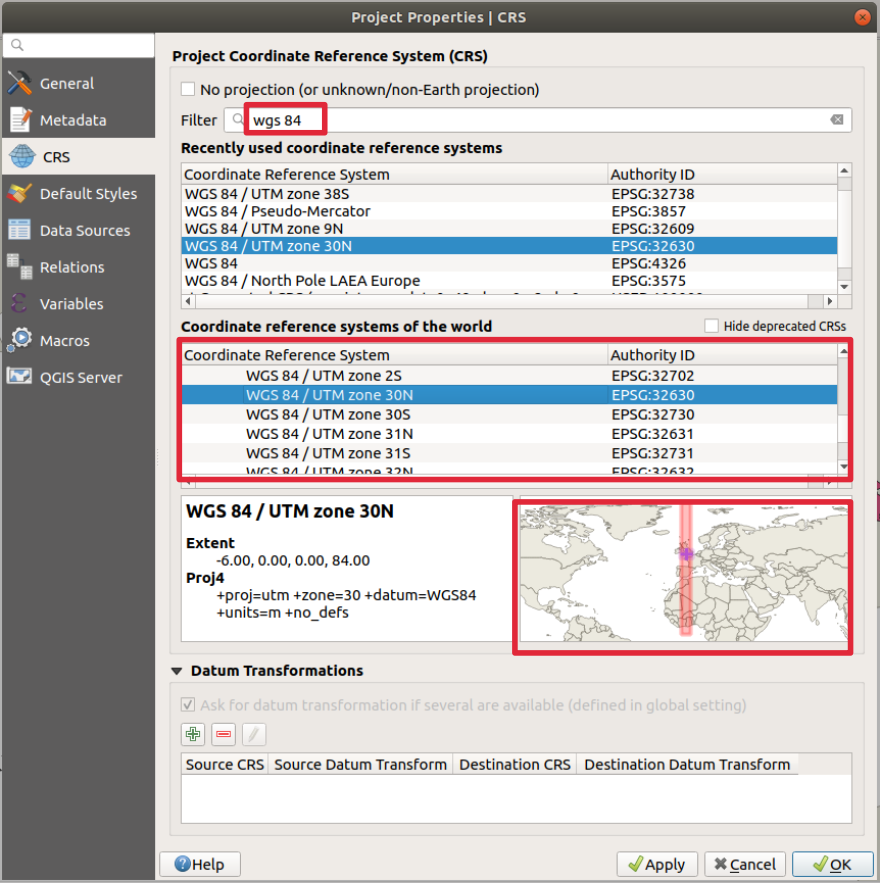
\includegraphics[width=0.6\textwidth]{images/project_properties_window_crs.png}
	\caption{Project properties window, selecting a different Project Coordinate Reference System}
	\label{ft_fig_firstfig3}
\end{figure}

By changing the CRS (from EPSG 4326 to EPSG 32630), the visual representation of the UK now has more familiar proportions.

\begin{figure}[!h]
	\centering
	\begin{minipage}{0.4\textwidth}
		\centering
		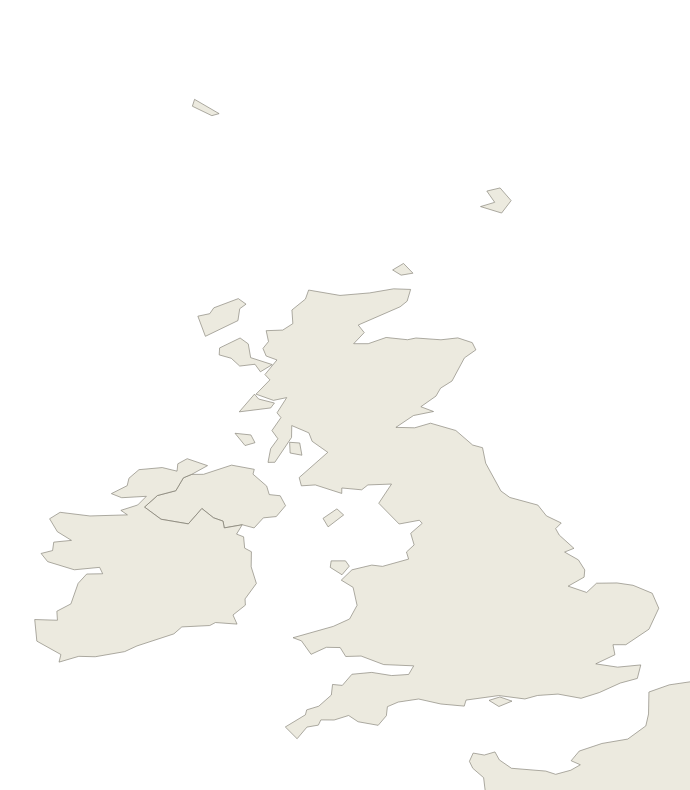
\includegraphics[width=0.8\textwidth]{images/uk_epsg4326.png}%epsg4326.png}%epsg4326_uk.png} % first figure itself
		\caption{The UK using projection EPSG 4326}
	\end{minipage}\hfill
	\begin{minipage}{0.35\textwidth}
		\centering
		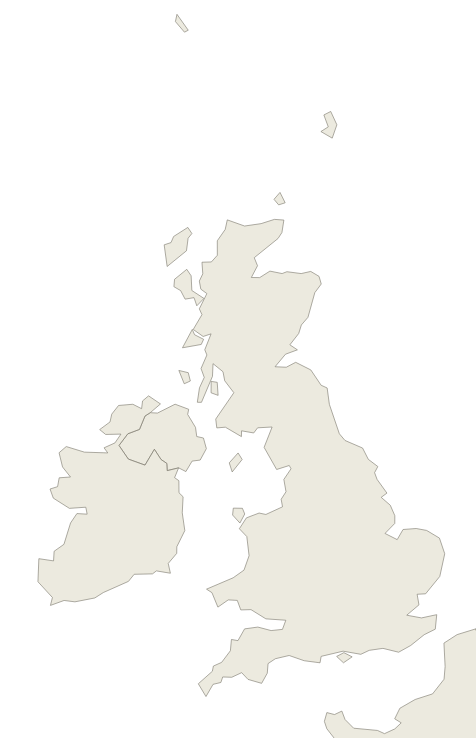
\includegraphics[width=0.7\textwidth]{images/uk_epsg32630.png}%epsg32630_uk.png} % second figure itself
		\caption{The UK using projection EPSG 32630}
	\end{minipage}
\end{figure}

Zoom to the world layer, to see how poor this projection works on the global scale.

\begin{figure}[!h]
	\centering
	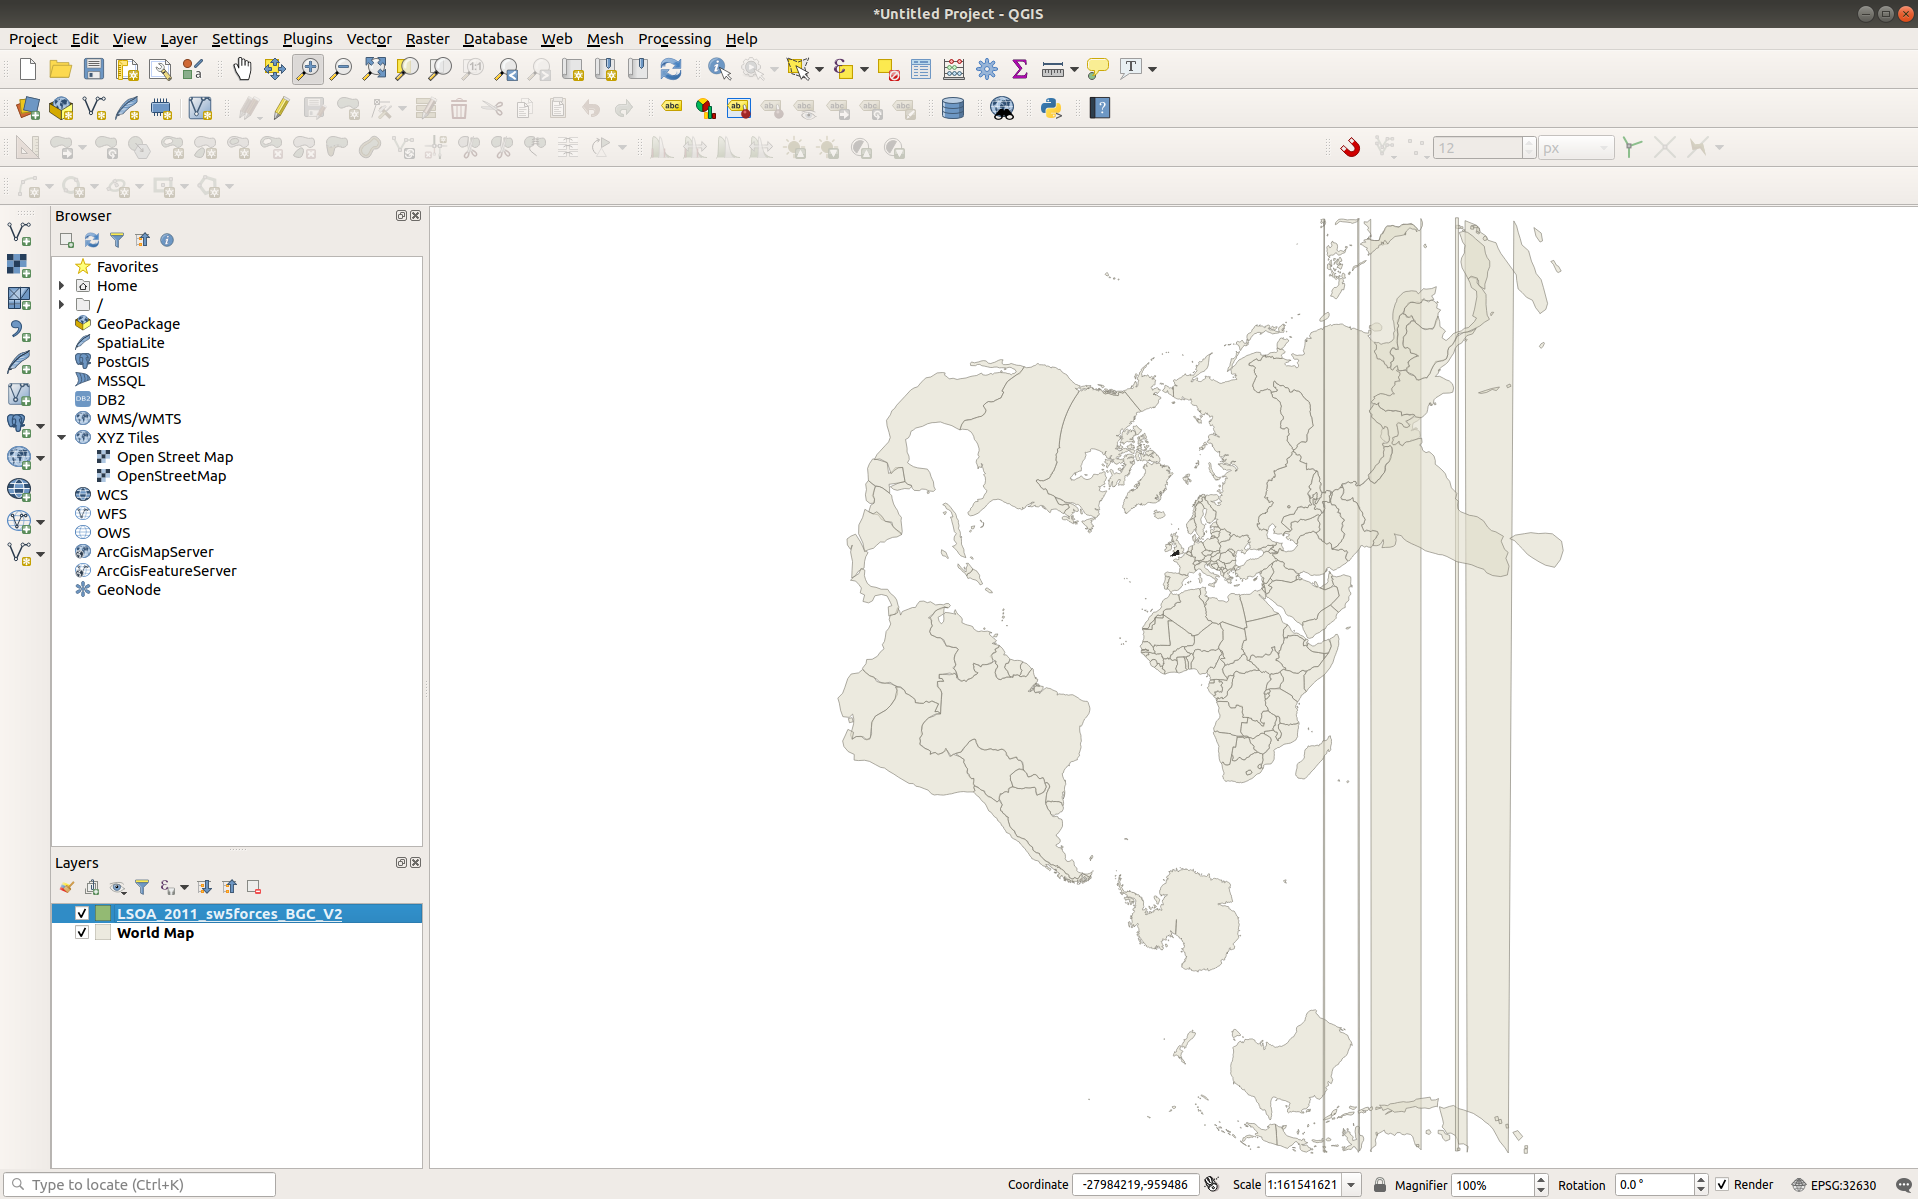
\includegraphics[width=0.5\textwidth]{images/world_map_EPSG32630.png}
	\caption{World map using projection EPSG 32630}
	\label{ft_fig_firstfig3}
\end{figure}

\textbf{Projections are also defined for each layer} in your project. If your layer does not have the correct projection it will not appear in the expected location on your map canvas.\\

To change the projection of a layer, right click on the layer name in the \emph{Layers} panel $\rightarrow$ Set CRS $\rightarrow$ Set layer CRS.\\

This will open a window very similar to the project properties window and allow you to specify a new projection for your layer.\\

Without more information about which is the correct projection, if the data is for the UK and is not projected onto the map canvas where I expect, I try changing it's projections to one of these:
\begin{enumerate}
	\item EPSG: 4326
	\item EPSG: 32630
	\item EPSG: 27700
	\item USER: 100000
\end{enumerate}
%Can now delete the world layer: right click on layer's name in the \textit{Layers Panel} and select \textit{Remove Layer}. Should now just have our one shapefile ($LSOA\_2011\_sw5forces\_BGC\_V2.shp$.) listed in the \textit{Layers Panel}.

%\begin{figure}[!h]
%	\centering
%	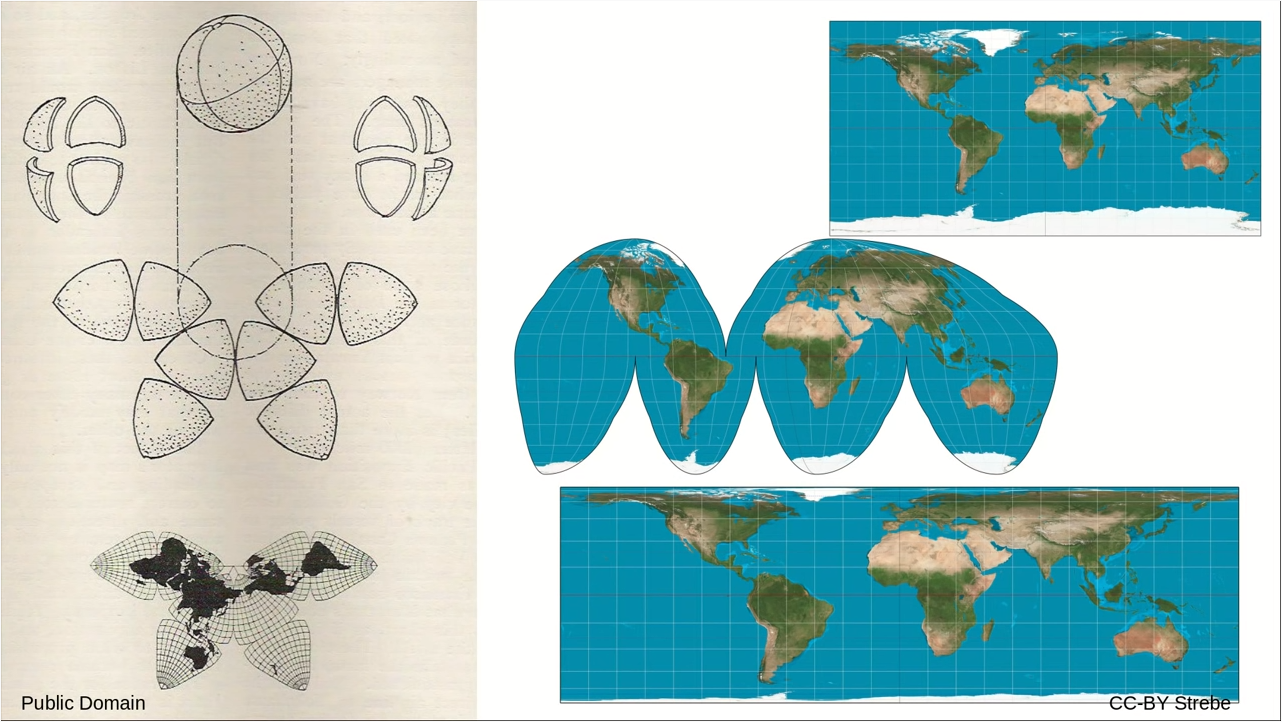
\includegraphics[width=0.8\textwidth]{images/3d_earth_to_2d_paper}
%	\caption{}
%	\label{ft_fig_firstfig3}
%\end{figure}